%%%%%%%%%%%%%%%%%%%%%%%%%%%%%%%%%%%%%%%%%%%%%%%%%%%%%%%%%%%%%%%%%%%%%%%% 
%%%%%%%%%%%%%%%%%%%%%%%%%%%%%%%%%%%%%%%%%%%%%%%%%%%%%%%%%%%%%%%%%%%%%%%% 
\begin{frame}
  \frametitle{IBM Power8 / Nvidia Pascal P100}

  \begin{itemize}
  \item {\bf \textcolor{violet}{Kokkos training material archive} (last up-to-date version) is on \texttt{ouessant}:}\\
    \myurl{/pwrwork/workshops/patc-201805/kokkos/training_kokkos.tar.gz}
  \item Use material from IBM/NVidia~\footnote{Thanks to Nicolas Tallet (IBM)}, gives detail on the platform\\
      See file: \myurl{doc/ouessant/Introduction.pdf} in archive
    \item Minimal information about software environment, how to build and run an application, submit a job on machine \texttt{ouessant}\\
      See file: \myurl{doc/ouessant/Ouessant-Application_User_Guide-16-12-1.pdf}
  \end{itemize}

\end{frame}

%%%%%%%%%%%%%%%%%%%%%%%%%%%%%%%%%%%%%%%%%%%%%%%%%%%%%%%%%%%%%%%%%%% 
%%%%%%%%%%%%%%%%%%%%%%%%%%%%%%%%%%%%%%%%%%%%%%%%%%%%%%%%%%%%%%%%%%% 
%%%%%%%%%%%%%%%%%%%%%%%%%%%%%%%%%%%%%%%%%%%%%%%%%%%%%%%%%%%%%%%%%%% 
\begin{frame}
  \frametitle{Kokkos: a programming model for performance portability}

  \only<1>{
    \begin{itemize}
    \item \textcolor{blue}{\textbf{Kokkos}} is a \textbf{C++ library} with \textcolor{red}{\textbf{parallel algorithmic patterns}} AND \textcolor{red}{\textbf{data containers}} for \textcolor{blue}{\textbf{node-level parallelism}}.
    \item Implementation relies heavily on \textbf{meta-programing} to derive native {\bf low-level code (OpenMP, Pthreads, CUDA, ...)} and adapt data structure {\bf memory layout} at compile-time
    \item Core developers at \textcolor{violet}{\bf SANDIA NL} (\textbf{H.C. Edwards, C. Trott})
    \end{itemize}
  }
  \only<2>{
    \begin{itemize}
    \item \textcolor{darkgreen}{\textbf{Open source}}, \myurl{https://github.com/kokkos/kokkos}
    \item Primarily developped as a base building layer for \textbf{generic high-performance parallel linear algebra} in \myhref{https://github.com/trilinos/Trilinos}{Trilinos}
    \item Also used in molecular dynamics code, e.g. \myhref{http://lammps.sandia.gov/}{LAMMPS}
    \item Goal: \textcolor{orange}{\textbf{ISO/C++ 2020 Standard}} subsumes Kokkos abstractions
    \end{itemize}
  }
  \begin{center}
    \includegraphics<1-2>[width=7cm]{doc/perf_portability/kokkos_summary}
  \end{center}

\end{frame}

%%%%%%%%%%%%%%%%%%%%%%%%%%%%%%%%%%%%%%%%%%%%%%%%%%%%%%%%%%%%%%%%%%% 
%%%%%%%%%%%%%%%%%%%%%%%%%%%%%%%%%%%%%%%%%%%%%%%%%%%%%%%%%%%%%%%%%%% 
%%%%%%%%%%%%%%%%%%%%%%%%%%%%%%%%%%%%%%%%%%%%%%%%%%%%%%%%%%%%%%%%%%% 
\begin{frame}
  \frametitle{Kokkos: a programming model for performance portability}

  \begin{center}
    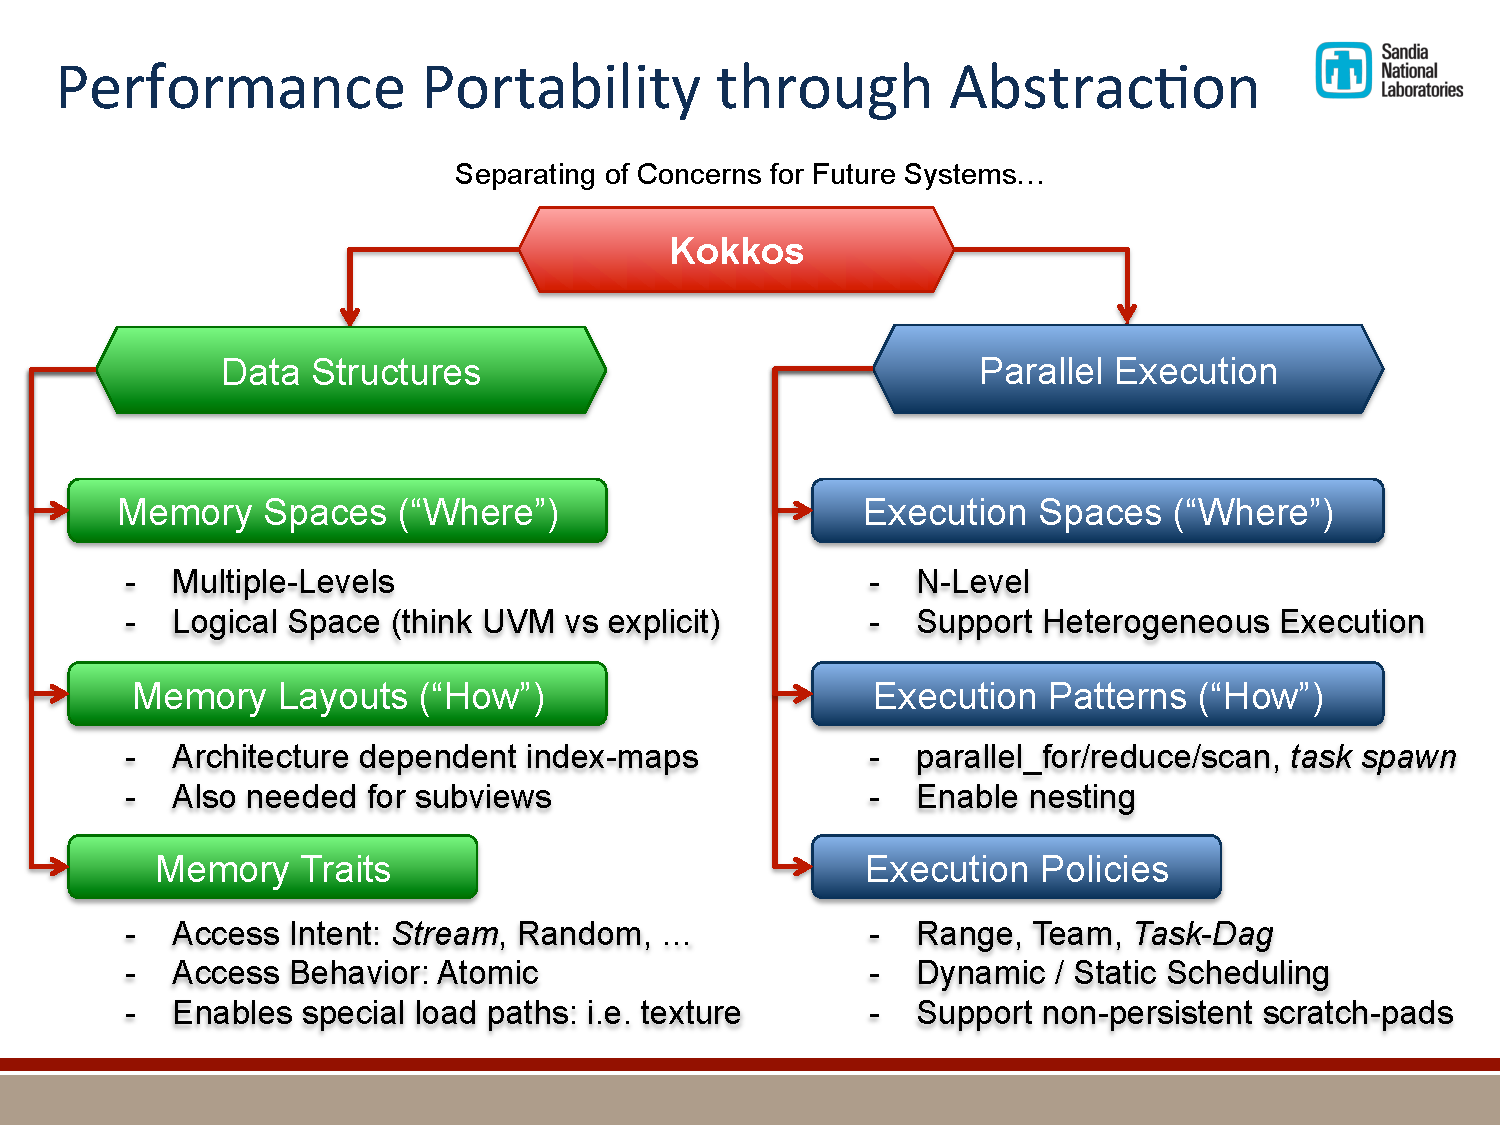
\includegraphics[width=8.5cm]{../intro/images/Kokkos-Multi-CoE_slide3}
  \end{center}

  {\small reference: \myurl{https://cfwebprod.sandia.gov/cfdocs/CompResearch/docs/Kokkos-Multi-CoE.pdf}}

\end{frame}

